\subsection{Cross validation}

For \textbf{$k$-fold cross-validation}\sidenote{$k$-fold cross-validation}, we consider different parts of the dataset for testing, as can be seen in \ref{fig:7_kfold_cv}. If the accuracy stays stable, one knows that the model is probably good and doesn't depend on certain parts of the training set.
\begin{itemize}
  \item Rule of thumb: typically $10$ is a good number for $k$
\end{itemize}

\begin{figure}[H]
  \centering
  \begin{subfigure}{0.5\textwidth}
    \centering
    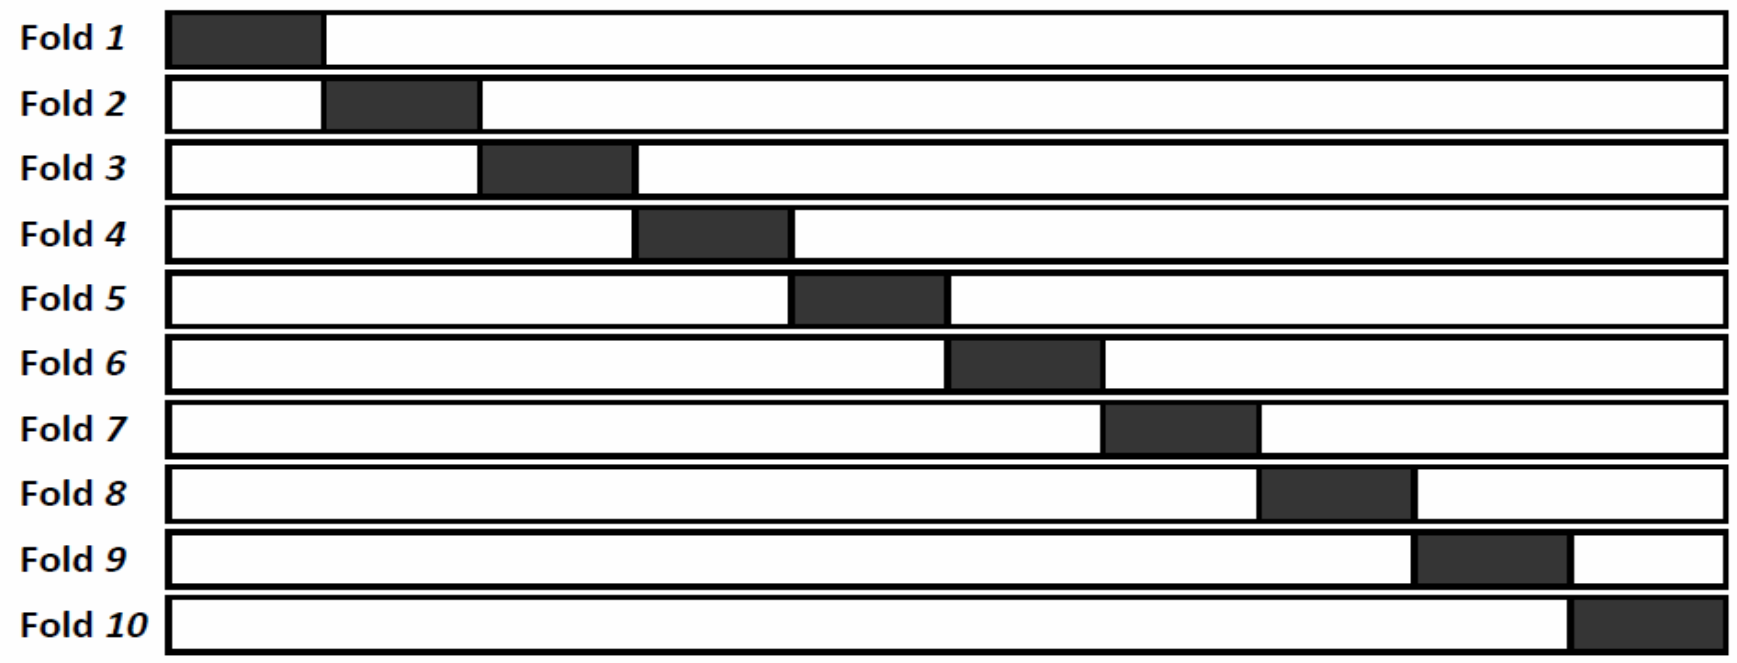
\includegraphics[width=\textwidth]{assets/sl/cross_val__kfold_set.png}
    \subcaption*{Split of test set (dark parts) for folds, light parts are training data}
  \end{subfigure}
  \hspace*{0.05\textwidth}
  \begin{subfigure}{0.4\textwidth}
    \centering
    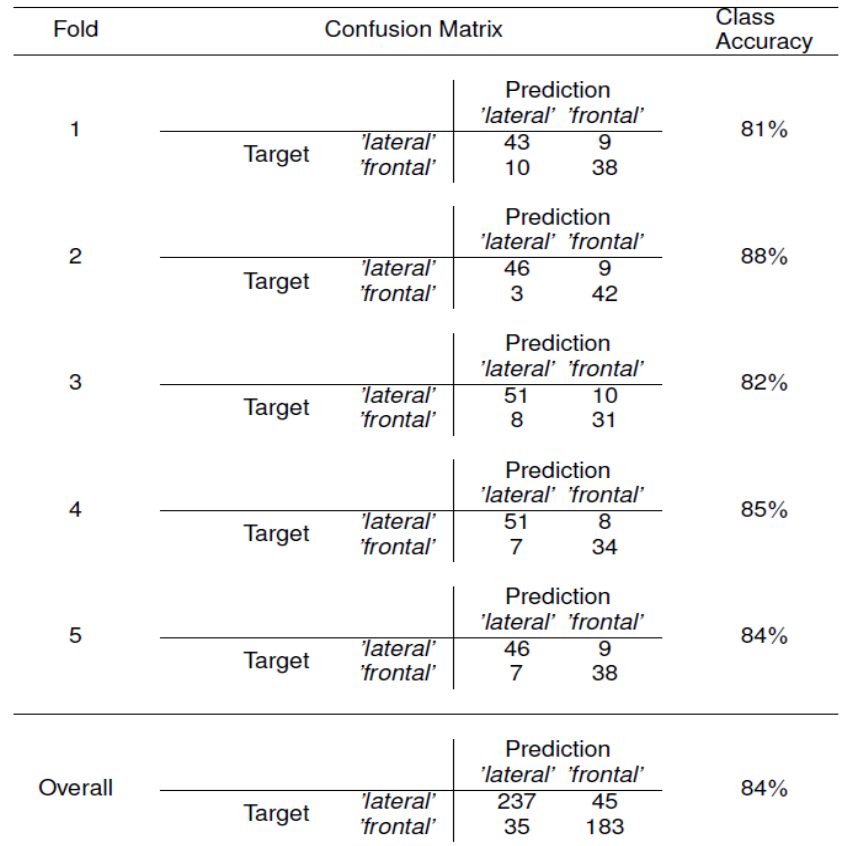
\includegraphics[width=\textwidth]{assets/sl/cross_val__kfold_res.png}
    \subcaption*{Result of 5-fold cross validation}
  \end{subfigure}

  \caption{$k$-fold cross-validation}
  \label{fig:7_kfold_cv}
\end{figure}

One special case of $k$-fold cross-validation is \textbf{leave-one-out cross-validation}\sidenote{Leave-one-out cross-validation} where $k=1$.
\begin{itemize}
  \item This is also known as \textbf{jackknifing}
  \item The test set is then only a single instance, and the approach is only used when less data is available
\end{itemize}

\begin{figure}[H]
  \centering
  \begin{subfigure}{0.6\textwidth}
    \centering
    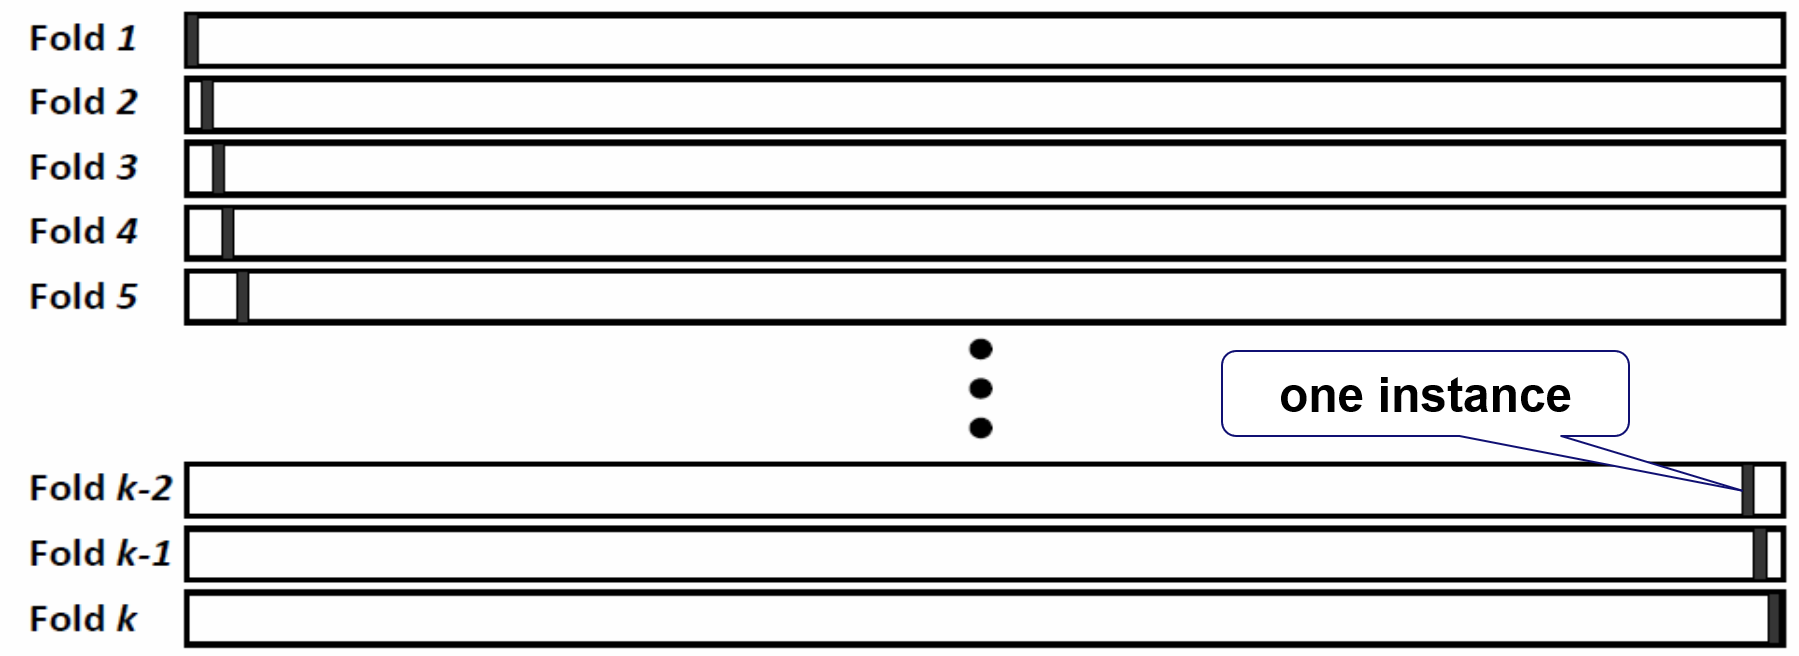
\includegraphics[width=\textwidth]{assets/sl/cross_val__1fold.png}
  \end{subfigure}

  \caption{Leave-one-out cross-validation}
  \label{fig:7_1fold_cv}
\end{figure}

Another cross-validation technique is \textbf{bootstrapping}\sidenote{Bootstrapping} where Repeatedly ($k$ times), $m$ random instances are selected as test set. 
\begin{itemize}
  \item This is typically used for smaller data sets, but $k$ is usually much higher than for the $k$-fold technique
\end{itemize}

\begin{figure}[H]
  \centering
  \begin{subfigure}{0.6\textwidth}
    \centering
    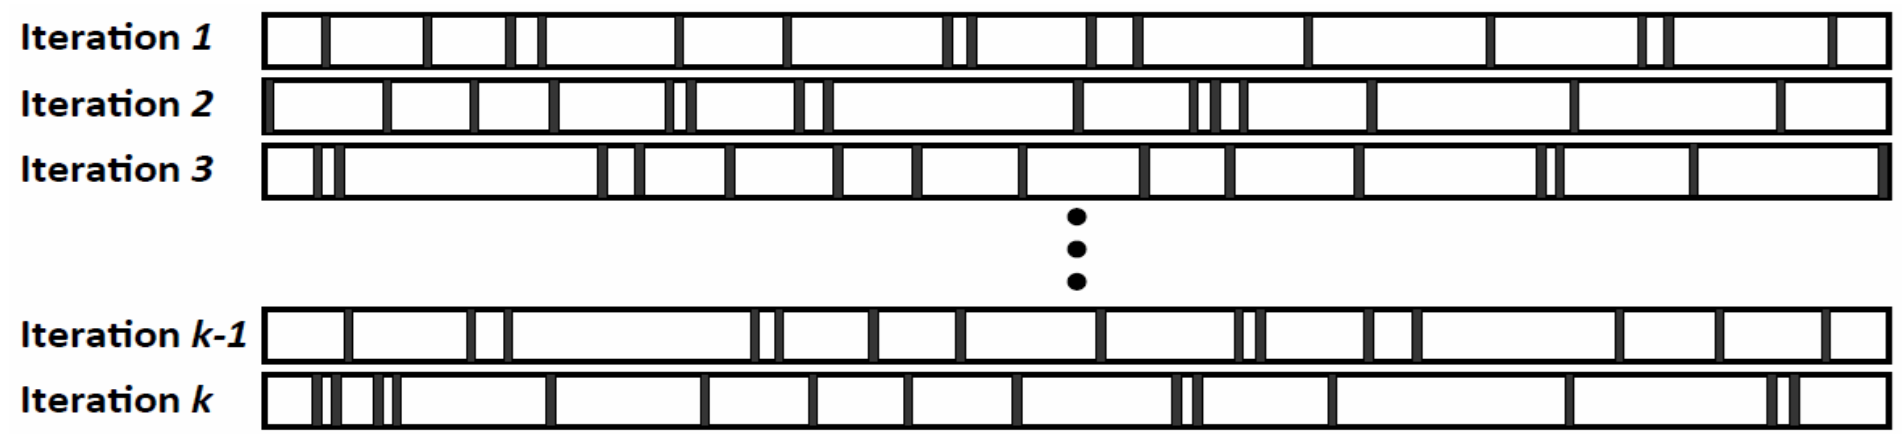
\includegraphics[width=\textwidth]{assets/sl/cross_val__bootstrapping.png}
  \end{subfigure}

  \caption{Bootstrapping}
  \label{fig:7_bootstrapping}
\end{figure}

Next, we'll compare random and out-of-time sampling.
\begin{itemize}
  \item For \textbf{randomm sampling}\sidenote{Random sampling} it goes that it works best if the instances are independent.
  \item But in the case of \textbf{context drift}, the time dimension plays a key role \begin{note}(imagine seasonal effects, backlog, ...)\end{note}
  \item $\rightarrow$ random sampling gives misleading good results if processes drift
  \item $\rightarrow$ use data from an entirely different time period, which is called \textbf{out-of-time sampling}\sidenote{Out-of-time sampling}
\end{itemize}

\begin{figure}[H]
  \centering
  \begin{subfigure}{0.5\textwidth}
    \centering
    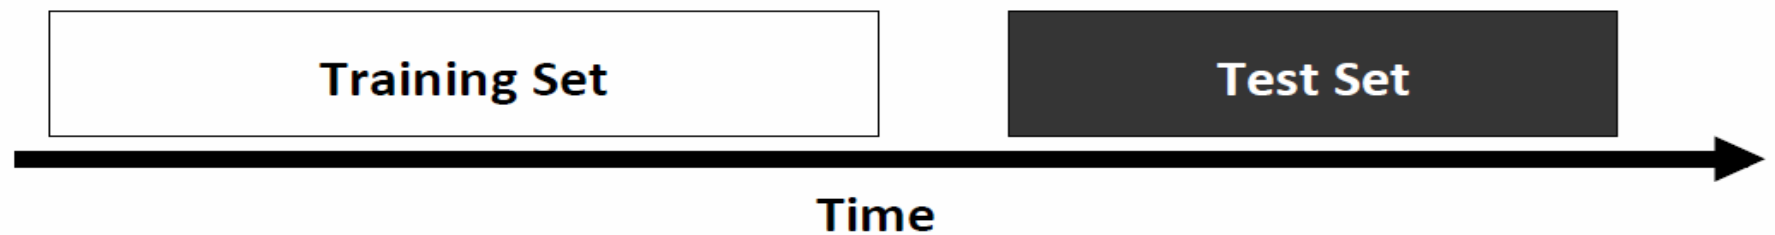
\includegraphics[width=\textwidth]{assets/sl/cross_val__out_of_time_concept.png}
    \subcaption*{Idea of out-of-time sampling}
  \end{subfigure}

  \vspace*{0.5cm}
  \begin{subfigure}{\textwidth}
    \centering
    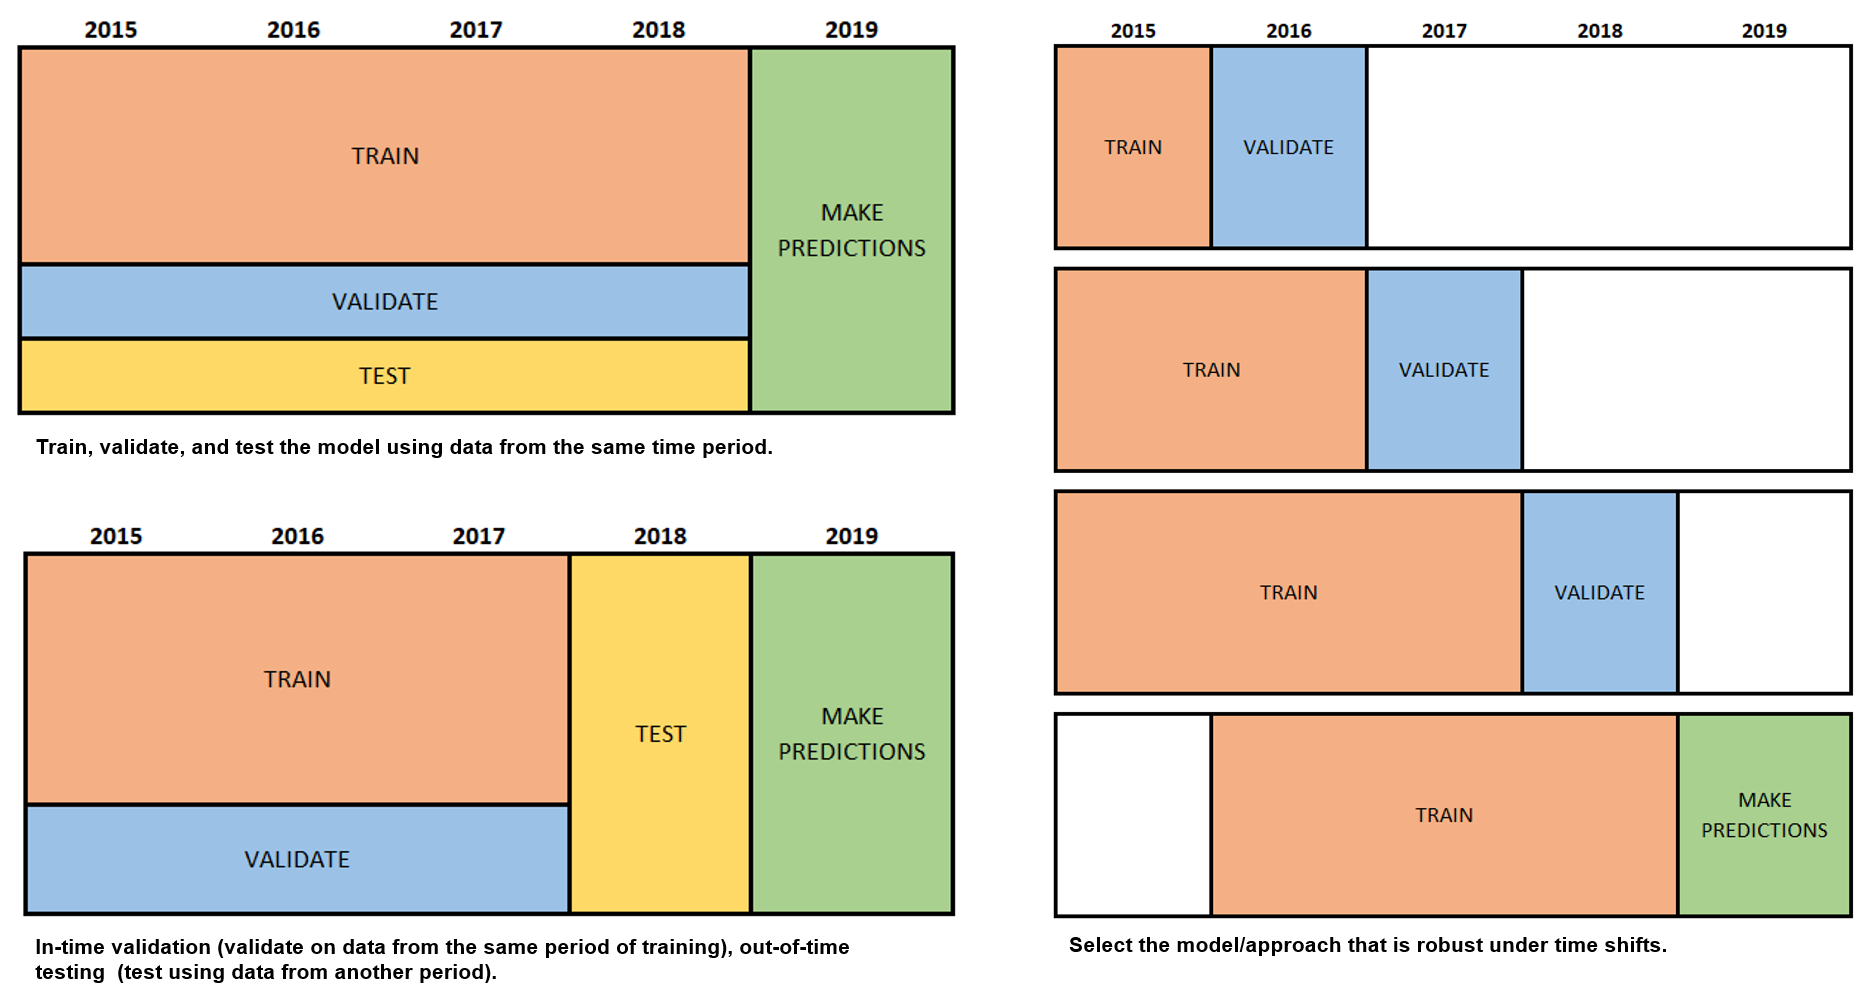
\includegraphics[width=\textwidth]{assets/sl/cross_val__out_of_time_model_models.png}
    \subcaption*{Different combinations (can train multiple models and select best one)}
  \end{subfigure}

  \vspace*{0.5cm}
  \begin{subfigure}{0.47\textwidth}
    \centering
    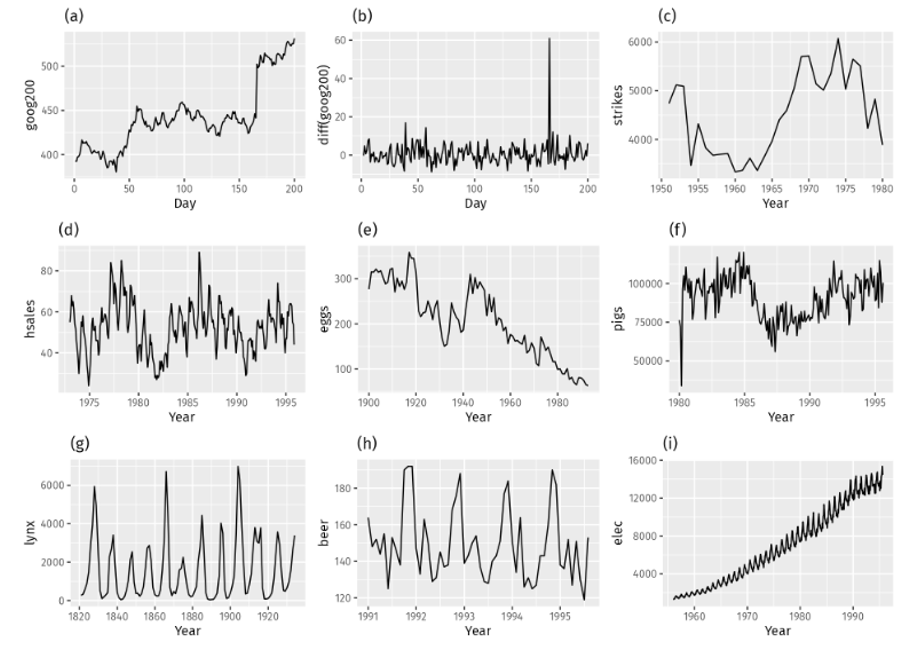
\includegraphics[width=\textwidth]{assets/sl/cross_val__out_of_time_model_drift.png}
  \end{subfigure}
  \hspace*{0.05\textwidth}
  \begin{subfigure}{0.47\textwidth}
    \centering
    \begin{itemize}
      \item \text{Models may degrade over time due to drifts}
      \item $\rightarrow$ \text{need to decide if and when to retrain the model}
      \item \text{Tradeoff: having enough data} $\leftrightarrow$ \text{adapting to trends}
    \end{itemize}
  \end{subfigure}

  \caption{Concept drift}
  \label{fig:7_concept_drift}
\end{figure}


